\subsection{The Ambient Calculus and the Obliq Programming Language}
\label{sec:ambient}

\subsubsection{The Ambient Calculus}
The ambient calculus provides a formal basis for describing mobility in concurrent systems.  Here mobility refers to both {\it{mobile\ computing}} (computation carried out in mobile devices) and {\it{mobile\ computation}} (code moves between the network sites) \citep{Cardelli98mobileambients}.  In reality, there is an additional security requirement for mobility, that is, the authorization for an agent to enter or exit certain administrative domain (e.g. a firewall).  The ambient calculus solves the above problems with a fundamental concept: ambient.  The three key attributes of a ambient are:
\begin{itemize}
  \item a name for access control (enter, exit, and open the ambient).
  \item a collection of local processes/agents that control the ambient.  
  \item a collection of sub-ambients. 
\end{itemize}

An atomic computation in the ambient calculus is a one-step movement of an ambient.  Although the pure ambient calculus with mobility is Turing-complete \citep{Cardelli98mobileambients}, communication primitives are necessary to comfort the encoding of other communication based calculi such as the $\pi$-calculus.  The full calculus is given through Table \ref{ambient-syn} to \ref{ambient-red}, cited from \citep{Cardelli98mobileambients}.  It is important to note that communication in the ambient calculus are local.  In other words, value (name or capability) communication only happens between two processes inside the same ambient.

\begin{table} [p]
  \begin{center}
  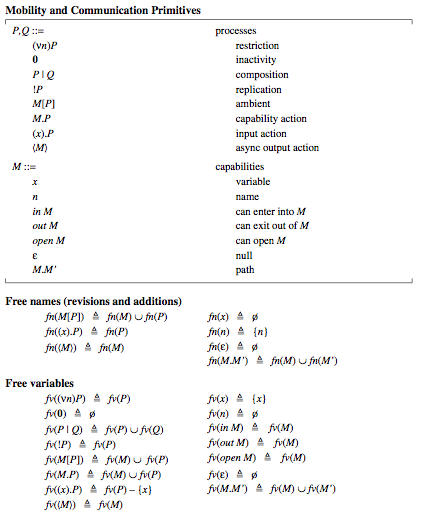
\includegraphics[scale=1]{ambient.png}
  \end{center}
  \captionsetup{justification=centering}  
  \caption{Syntax and scope in the ambient-calculus \\ -- \citep{Cardelli98mobileambients}}
  \label{ambient-syn}
\end{table}

\begin{table} [p]
  \begin{center}
  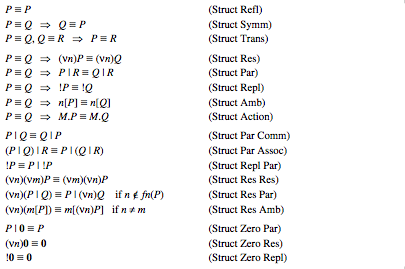
\includegraphics[scale=1]{ambient_str_1.png}
  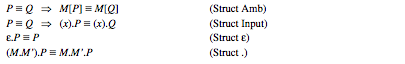
\includegraphics[scale=1]{ambient_str_2.png}
  \end{center}
  \captionsetup{justification=centering}    
  \caption{Structure congurence in the ambient-calculus \\ -- \citep{Cardelli98mobileambients}}
  \label{ambient-str}
\end{table}

\begin{table} [p]
  \begin{center}
  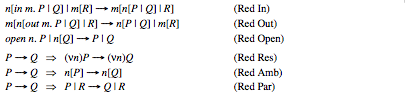
\includegraphics[scale=1]{ambient_red_1.png}
  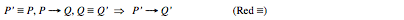
\includegraphics[scale=1]{ambient_red_2.png}
  
\includegraphics[scale=1]{ambient_red_3.png}
  \end{center}
  \captionsetup{justification=centering}    
  \caption{Reduction in the ambient-calculus \\ -- \citep{Cardelli98mobileambients}}
  \label{ambient-red}
\end{table}

\subsubsection{The Obliq Programming Language}
At the time of writing this report, there is no real language that implements the ambient-calculus\footnote{\citet{VMAmbient} proposed a virtual machine for the ambient calculus.}.  Instead,  this section will introduce the Obliq language, which has certain notions of ambient and influenced the design of the ambient calculus.

Obliq\citep{obliq} is one of the earliest programming languages which support distributed programming.  The language was designed before the pervasive of web applications.  It only supports simple object model which is a collection of fields.  Each field of an Obliq object could be a value (a constant or a procedure), a method, or an alias to an object.  An object could either be constructed directly by specifying its fields, or be cloned from other objects.  

The four operations which could be performed on objects are:
\begin{itemize}
  \item selection: a value field of a object could be selected and transmitted over the web.  If the selected value is a constant, the value will be transmitted.  By contrast, if the selected value is a method, values of its arguments will be transmitted to the remote site where the method is defined, the computation is performed remotely, and the result or an exception is returned to the site of the selection.
  \item updating: when an updating operation is performed on an remote object, the selected filed is updated to a value that might be sent across the web.  If the selected filed is a method, a transmission of method closure is required.
  \item cloning: cloning an object will yield a new object which contains all fields of argument objects or raise an error if field names of argument objects conflict.
  \item aliasing:  After executing an aliasing method, a.x := $\bf{alias}$ y $\bf{of}$ b $\bf{end}$, further operations on x of a will be redirected to y of b.
\end{itemize}

It is important to note that Obliq, as some other languages in the pre-web era, does not distinguish local values from distributed values.  By contrast, \citet{dis_note} pointed out that distinct views must be adopted for local and distributed objects, due to differences in latency, memory access, partial failure, and concurrency.